\documentclass[14pt]{extbook}
\usepackage{multicol, enumerate, enumitem, hyperref, color, soul, setspace, parskip, fancyhdr} %General Packages
\usepackage{amssymb, amsthm, amsmath, latexsym, units, mathtools} %Math Packages
\everymath{\displaystyle} %All math in Display Style
% Packages with additional options
\usepackage[headsep=0.5cm,headheight=12pt, left=1 in,right= 1 in,top= 1 in,bottom= 1 in]{geometry}
\usepackage[usenames,dvipsnames]{xcolor}
\usepackage{dashrule}  % Package to use the command below to create lines between items
\newcommand{\litem}[1]{\item#1\hspace*{-1cm}\rule{\textwidth}{0.4pt}}
\pagestyle{fancy}
\lhead{Progress Quiz 10}
\chead{}
\rhead{Version B}
\lfoot{5170-5105}
\cfoot{}
\rfoot{Summer C 2021}
\begin{document}

\begin{enumerate}
\litem{
Solve the linear equation below. Then, choose the interval that contains the solution.\[ \frac{-4x -7}{7} - \frac{3x -5}{4} = \frac{-9x + 8}{5} \]\begin{enumerate}[label=\Alph*.]
\item \( x \in [2.82, 5.82] \)
\item \( x \in [19.9, 22.9] \)
\item \( x \in [-0.32, 2.68] \)
\item \( x \in [7.04, 13.04] \)
\item \( \text{There are no real solutions.} \)

\end{enumerate} }
\litem{
Write the equation of the line in the graph below in Standard Form $Ax+By=C$. Then, choose the intervals that contain $A, B, \text{ and } C$.
\begin{center}
    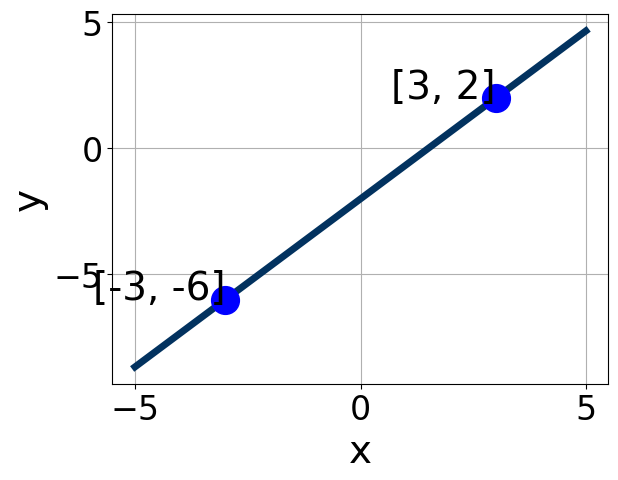
\includegraphics[width=0.5\textwidth]{../Figures/linearGraphToStandardCopyB.png}
\end{center}
\begin{enumerate}[label=\Alph*.]
\item \( A \in [-3.2, -0.6], \hspace{3mm} B \in [-0.47, 2.53], \text{ and } \hspace{3mm} C \in [-2.6, -1.5] \)
\item \( A \in [3.6, 4.2], \hspace{3mm} B \in [-4.11, -1.78], \text{ and } \hspace{3mm} C \in [5.4, 7.9] \)
\item \( A \in [-3.2, -0.6], \hspace{3mm} B \in [-1.64, 0.98], \text{ and } \hspace{3mm} C \in [1.9, 4] \)
\item \( A \in [-4.8, -3], \hspace{3mm} B \in [2.28, 3.26], \text{ and } \hspace{3mm} C \in [-9.4, -4.7] \)
\item \( A \in [3.6, 4.2], \hspace{3mm} B \in [2.28, 3.26], \text{ and } \hspace{3mm} C \in [-9.4, -4.7] \)

\end{enumerate} }
\litem{
Find the equation of the line described below. Write the linear equation in the form $ y=mx+b $ and choose the intervals that contain $m$ and $b$.\[ \text{Perpendicular to } 6 x - 7 y = 6 \text{ and passing through the point } (7, -2). \]\begin{enumerate}[label=\Alph*.]
\item \( m \in [-0.91, -0.66] \hspace*{3mm} b \in [2, 6.5] \)
\item \( m \in [-1.52, -1.16] \hspace*{3mm} b \in [2, 6.5] \)
\item \( m \in [-1.52, -1.16] \hspace*{3mm} b \in [-9.4, -7.3] \)
\item \( m \in [1.14, 1.33] \hspace*{3mm} b \in [-10.2, -9.8] \)
\item \( m \in [-1.52, -1.16] \hspace*{3mm} b \in [-7.6, -5.5] \)

\end{enumerate} }
\litem{
Solve the equation below. Then, choose the interval that contains the solution.\[ -11(-8x + 10) = -6(-13x + 17) \]\begin{enumerate}[label=\Alph*.]
\item \( x \in [20.5, 21.5] \)
\item \( x \in [0.2, 1] \)
\item \( x \in [-22.5, -20.4] \)
\item \( x \in [1.1, 2.2] \)
\item \( \text{There are no real solutions.} \)

\end{enumerate} }
\litem{
Find the equation of the line described below. Write the linear equation in the form $ y=mx+b $ and choose the intervals that contain $m$ and $b$.\[ \text{Parallel to } 7 x - 6 y = 12 \text{ and passing through the point } (2, -9). \]\begin{enumerate}[label=\Alph*.]
\item \( m \in [0.76, 1.05] \hspace*{3mm} b \in [-11.78, -11.17] \)
\item \( m \in [1.13, 1.3] \hspace*{3mm} b \in [11.14, 11.58] \)
\item \( m \in [-1.45, -1.1] \hspace*{3mm} b \in [-7.04, -6.43] \)
\item \( m \in [1.13, 1.3] \hspace*{3mm} b \in [-11.01, -10.53] \)
\item \( m \in [1.13, 1.3] \hspace*{3mm} b \in [-11.78, -11.17] \)

\end{enumerate} }
\litem{
Solve the linear equation below. Then, choose the interval that contains the solution.\[ \frac{7x -8}{5} - \frac{5x + 4}{7} = \frac{4x -7}{8} \]\begin{enumerate}[label=\Alph*.]
\item \( x \in [-1.08, 0.3] \)
\item \( x \in [0.51, 0.88] \)
\item \( x \in [26.71, 27.58] \)
\item \( x \in [6.5, 7.26] \)
\item \( \text{There are no real solutions.} \)

\end{enumerate} }
\litem{
First, find the equation of the line containing the two points below. Then, write the equation in the form $ y=mx+b $ and choose the intervals that contain $m$ and $b$.\[ (-9, -8) \text{ and } (-10, 3) \]\begin{enumerate}[label=\Alph*.]
\item \( m \in [-13, -7] \hspace*{3mm} b \in [107, 110] \)
\item \( m \in [5, 13] \hspace*{3mm} b \in [110, 116] \)
\item \( m \in [-13, -7] \hspace*{3mm} b \in [13, 19] \)
\item \( m \in [-13, -7] \hspace*{3mm} b \in [-113, -106] \)
\item \( m \in [-13, -7] \hspace*{3mm} b \in [0, 4] \)

\end{enumerate} }
\litem{
Write the equation of the line in the graph below in Standard Form $Ax+By=C$. Then, choose the intervals that contain $A, B, \text{ and } C$.
\begin{center}
    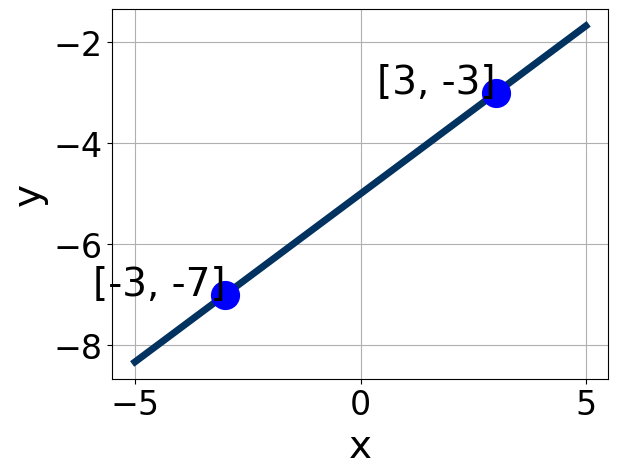
\includegraphics[width=0.5\textwidth]{../Figures/linearGraphToStandardB.png}
\end{center}
\begin{enumerate}[label=\Alph*.]
\item \( A \in [-0.9, -0.3], \hspace{3mm} B \in [-1.86, -0.87], \text{ and } \hspace{3mm} C \in [3, 12] \)
\item \( A \in [-0.9, -0.3], \hspace{3mm} B \in [0.8, 2.46], \text{ and } \hspace{3mm} C \in [-11, -4] \)
\item \( A \in [0.5, 2.3], \hspace{3mm} B \in [1.88, 3.18], \text{ and } \hspace{3mm} C \in [-20, -12] \)
\item \( A \in [-5.1, -1.8], \hspace{3mm} B \in [1.88, 3.18], \text{ and } \hspace{3mm} C \in [-20, -12] \)
\item \( A \in [0.5, 2.3], \hspace{3mm} B \in [-3.74, -2.96], \text{ and } \hspace{3mm} C \in [12, 16] \)

\end{enumerate} }
\litem{
First, find the equation of the line containing the two points below. Then, write the equation in the form $ y=mx+b $ and choose the intervals that contain $m$ and $b$.\[ (-7, -10) \text{ and } (4, -5) \]\begin{enumerate}[label=\Alph*.]
\item \( m \in [-1.05, -0.36] \hspace*{3mm} b \in [-3.31, -3.02] \)
\item \( m \in [0.14, 0.87] \hspace*{3mm} b \in [6.13, 6.98] \)
\item \( m \in [0.14, 0.87] \hspace*{3mm} b \in [-9.15, -8.92] \)
\item \( m \in [0.14, 0.87] \hspace*{3mm} b \in [-6.97, -6.66] \)
\item \( m \in [0.14, 0.87] \hspace*{3mm} b \in [-3.08, -2.79] \)

\end{enumerate} }
\litem{
Solve the equation below. Then, choose the interval that contains the solution.\[ -17(-4x -5) = -16(-12x + 19) \]\begin{enumerate}[label=\Alph*.]
\item \( x \in [-2.58, -1.04] \)
\item \( x \in [0.12, 1.3] \)
\item \( x \in [0.92, 2.31] \)
\item \( x \in [2.37, 3.57] \)
\item \( \text{There are no real solutions.} \)

\end{enumerate} }
\end{enumerate}

\end{document}